% Import default values & document settings
% Layout settings
\newcommand{\FIITdefaultFontSize}[0] {12pt}
\setcounter{secnumdepth}{3}
\setcounter{tocdepth}{3}

% Language settings
\newcommand{\FIITlanguage}[0] {slovak}
%\def\FIITlagEN{}

% Global texts
\newcommand{\FIITuniversity}[0] {Slovak University of Technology in Bratislava}
\newcommand{\FIITuniversitySK}[0] {Slovenská Technická Univerzita v Bratislave}
\newcommand{\FIITfaculty}[0] {Faculty of informatics and information technologies}
\newcommand{\FIITfacultySK}[0] {Fakulta informatiky a informačných technológií}
\newcommand{\FIITthesis}[0] {Bachelor's thesis}
\newcommand{\FIITthesisSK}[0] {Bakalárska práca}
\newcommand{\FIITtitle}[0] {Very important project}
\newcommand{\FIITtitleSK}[0] {Velmi dolezity projekt}
\newcommand{\FIITauthor}[0] {Jano Mrkvicka}
\newcommand{\FIITsupervisor}[0] {Peter Bandur}
\newcommand{\FIITevidenceNumber}[0] {FIIT-XXXX-XXXXX}
\newcommand{\FIITdate}[0] {December 2019}
\newcommand{\FIITdateSK}[0] {December 2019}
\newcommand{\FIITstudyProgram}[0] {Information Security}
\newcommand{\FIITstudyProgramSK}[0] {Informačná bezpečnosť}
\newcommand{\FIITstudyField}[0] {Computer Science}
\newcommand{\FIITdegreeCourseSK}[0] {9.2.1 Informatika}
\newcommand{\FIITinstitute}[0] {Institute of Computer Engineering and Applied Informatics}
\newcommand{\FIITinstituteSK}[0] {Ústav počítačového inžinierstva a aplikovanej informatiky}
\newcommand{\FIITsignPlace}[0] {In Bratislava, }
\newcommand{\FIITsignPlaceSK}[0] {V Bratislave, }
\newcommand{\FIITsignDate}[0] {8.2.2020}
\newcommand{\FIITArchiveName}[0] {BP\_prilohy\_digital\_JanoMrkvicka.zip}


% Setup document
\documentclass[\FIITdefaultFontSize,a4paper,twoside,openright,\FIITlanguage]{book}

% Load all necessary packages
\usepackage[final]{pdfpages}
\usepackage[utf8]{inputenc}
\usepackage[T1]{fontenc}
\usepackage[\FIITlanguage]{babel}
\usepackage[a4paper]{geometry}
\usepackage[
    left = \glqq,% 
    right = \grqq,% 
    leftsub = \glq,% 
    rightsub = \grq%
]{dirtytalk}
\usepackage[parfill]{parskip}
\usepackage{enumitem}
\usepackage{calc}
\usepackage{graphicx}
\usepackage{float}
\usepackage{longtable}
\usepackage{setspace}
\usepackage{tabularx}
\usepackage{fancyhdr}
\usepackage[backend=bibtex,sorting=none]{biblatex}
\usepackage{listing}
\usepackage{lscape}
\usepackage{afterpage}
\usepackage{hyperref}
%\usepackage{bera}
\usepackage{listings}
\usepackage{xcolor}
\usepackage{lipsum}
\usepackage{minted}
\usepackage{tikz}
\usepackage{tocloft}

% lscape.sty Produce landscape pages in a (mainly) portrait document.
\usepackage{lscape}

% Custom commands
\newcommand{\signaturespace}[2]{
  % #1 = width of the dotted line
  % #2 = legend
  \begingroup
  \renewcommand{\arraystretch}{0}
  \begin{tabular}[t]{cc}
  \hspace*{0pt}
  \cleaders\hbox{\kern.6pt.\kern.6pt}\hskip#1\relax
  \hspace*{0pt}
  \\[0.5cm]
  #2
  \end{tabular}
  \endgroup
}

\newcommand{\emptypage}{\newpage
\thispagestyle{empty}
\mbox{}
\newpage}

% openright does not work :(
\let\tmp\oddsidemargin
\let\oddsidemargin\evensidemargin
\let\evensidemargin\tmp
\reversemarginpar

\bibliography{bibliography}

% Page design
\pagestyle{fancy}
\lhead{\nouppercase{\leftmark}}
\chead{}
\rhead{}
\lfoot{}
\cfoot{\thepage}
\rfoot{}

\begin{document}

% Layout
\setstretch{1.5}

% Bibliography
\ifx\FIITlagEN\undefined
\defbibheading{references}[Zoznam použitej literatúry]{ 
  \chapter*{#1}
  \markboth{#1}{#1}
}
\else
\defbibheading{references}[References]{ 
  \chapter*{#1}
  \markboth{#1}{#1}
}
\fi

% Cover & title page
% Cover page
	\begin{center}
\thispagestyle{empty}
\ifx\FIITlagEN\undefined
{\Large \FIITuniversitySK}
\else
{\Large \FIITuniversity}
\fi
\par\end{center}{\Large \par}

\begin{center}
\ifx\FIITlagEN\undefined
{\Large \FIITfacultySK}
\else
{\Large \FIITfaculty}
\fi
\par\end{center}{\Large \par}

\smallskip{}

\begin{center}
\ifx\FIITlagEN\undefined
Evidenčné číslo: \FIITevidenceNumber
\else
Reg. No.: \FIITevidenceNumber
\fi
\par\end{center}
\vfill{}

\begin{center}
\textbf{\Large \FIITauthor}
\par\end{center}{\Large \par}

\medskip{}


\begin{center}
\ifx\FIITlagEN\undefined
\textbf{\LARGE \FIITtitleSK}
\else
\textbf{\LARGE \FIITtitle}
\fi
\par\end{center}{\huge \par}

\medskip{}


\begin{center}

\ifx\FIITlagEN\undefined
{\Large \FIITthesisSK}
\else
{\Large \FIITthesis}
\fi
\par\end{center}{\Large \par}

\vfill{}

\ifx\FIITlagEN\undefined
Vedúci práce: \FIITsupervisor
\else
Supervisor: \FIITsupervisor
\fi

\medskip{}

\ifx\FIITlagEN\undefined
\FIITdateSK
\else
\FIITdate
\fi

\pagenumbering{roman}
\emptypage





% Thesis title page
	\begin{center}
\thispagestyle{empty}
\ifx\FIITlagEN\undefined
{\Large \FIITuniversitySK}
\else
{\Large \FIITuniversity}
\fi
\par\end{center}{\Large \par}

\begin{center}
\ifx\FIITlagEN\undefined
{\Large \FIITfacultySK}
\else
{\Large \FIITfaculty}
\fi
\par\end{center}{\Large \par}

\smallskip{}

\begin{center}
\ifx\FIITlagEN\undefined
Evidenčné číslo: \FIITevidenceNumber
\else
Reg. No.: \FIITevidenceNumber
\fi
\par\end{center}
\vfill{}

\begin{center}
\textbf{\Large \FIITauthor}
\par\end{center}{\Large \par}

\medskip{}


\begin{center}
\ifx\FIITlagEN\undefined
\textbf{\LARGE \FIITtitleSK}
\else
\textbf{\LARGE \FIITtitle}
\fi
\par\end{center}{\huge \par}

\medskip{}


\begin{center}

\ifx\FIITlagEN\undefined
{\Large \FIITthesisSK}
\else
{\Large \FIITthesis}
\fi
\par\end{center}{\Large \par}

\vfill{}

\ifx\FIITlagEN\undefined
Študijný program: \FIITstudyProgramSK

Číslo a názov študijného odboru: \FIITdegreeCourseSK

Školiace pracovisko: \FIITinstituteSK

Vedúci práce: \FIITsupervisor
\else
Study program: \FIITstudyProgram

Degree course: \FIITdegreeCourse

Place of elaboration: \FIITinstitute

Supervisor: \FIITsupervisor
\fi

\medskip{}

\ifx\FIITlagEN\undefined
\FIITdateSK
\else
\FIITdate
\fi

\emptypage


% Annotation
% Annotation in English
\thispagestyle{empty}

\vspace*{\fill}

\section*{Annotation}

\begin{minipage}[t]{1\columnwidth}
\FIITuniversity

\FIITfaculty

Degree Course: \FIITstudyProgram\\

Author: \FIITauthor

\FIITthesis: \FIITtitle

Supervisor: \FIITsupervisor

\FIITdate
\end{minipage}

\bigskip{}

\lorem{3}

\newpage{}\thispagestyle{empty}

\newpage
\thispagestyle{empty}
\mbox{}
\newpage



% Annotation in Slovak
\thispagestyle{empty}

\vspace*{\fill}

\section*{Anotácia}

\begin{minipage}[t]{1\columnwidth}
\FIITuniversitySK

\FIITfacultySK

Študijný program: \FIITstudyProgramSK\\

Autor: \FIITauthor

\FIITthesisSK: \FIITtitleSK

Vedúci projektu: \FIITsupervisor

\FIITdateSK
\end{minipage}

\bigskip{}

\lorem{3}

\newpage{}\thispagestyle{empty}\medskip{}

\newpage
\thispagestyle{empty}
\mbox{}
\newpage



% Thesis assignment
\newpage
\thispagestyle{empty}
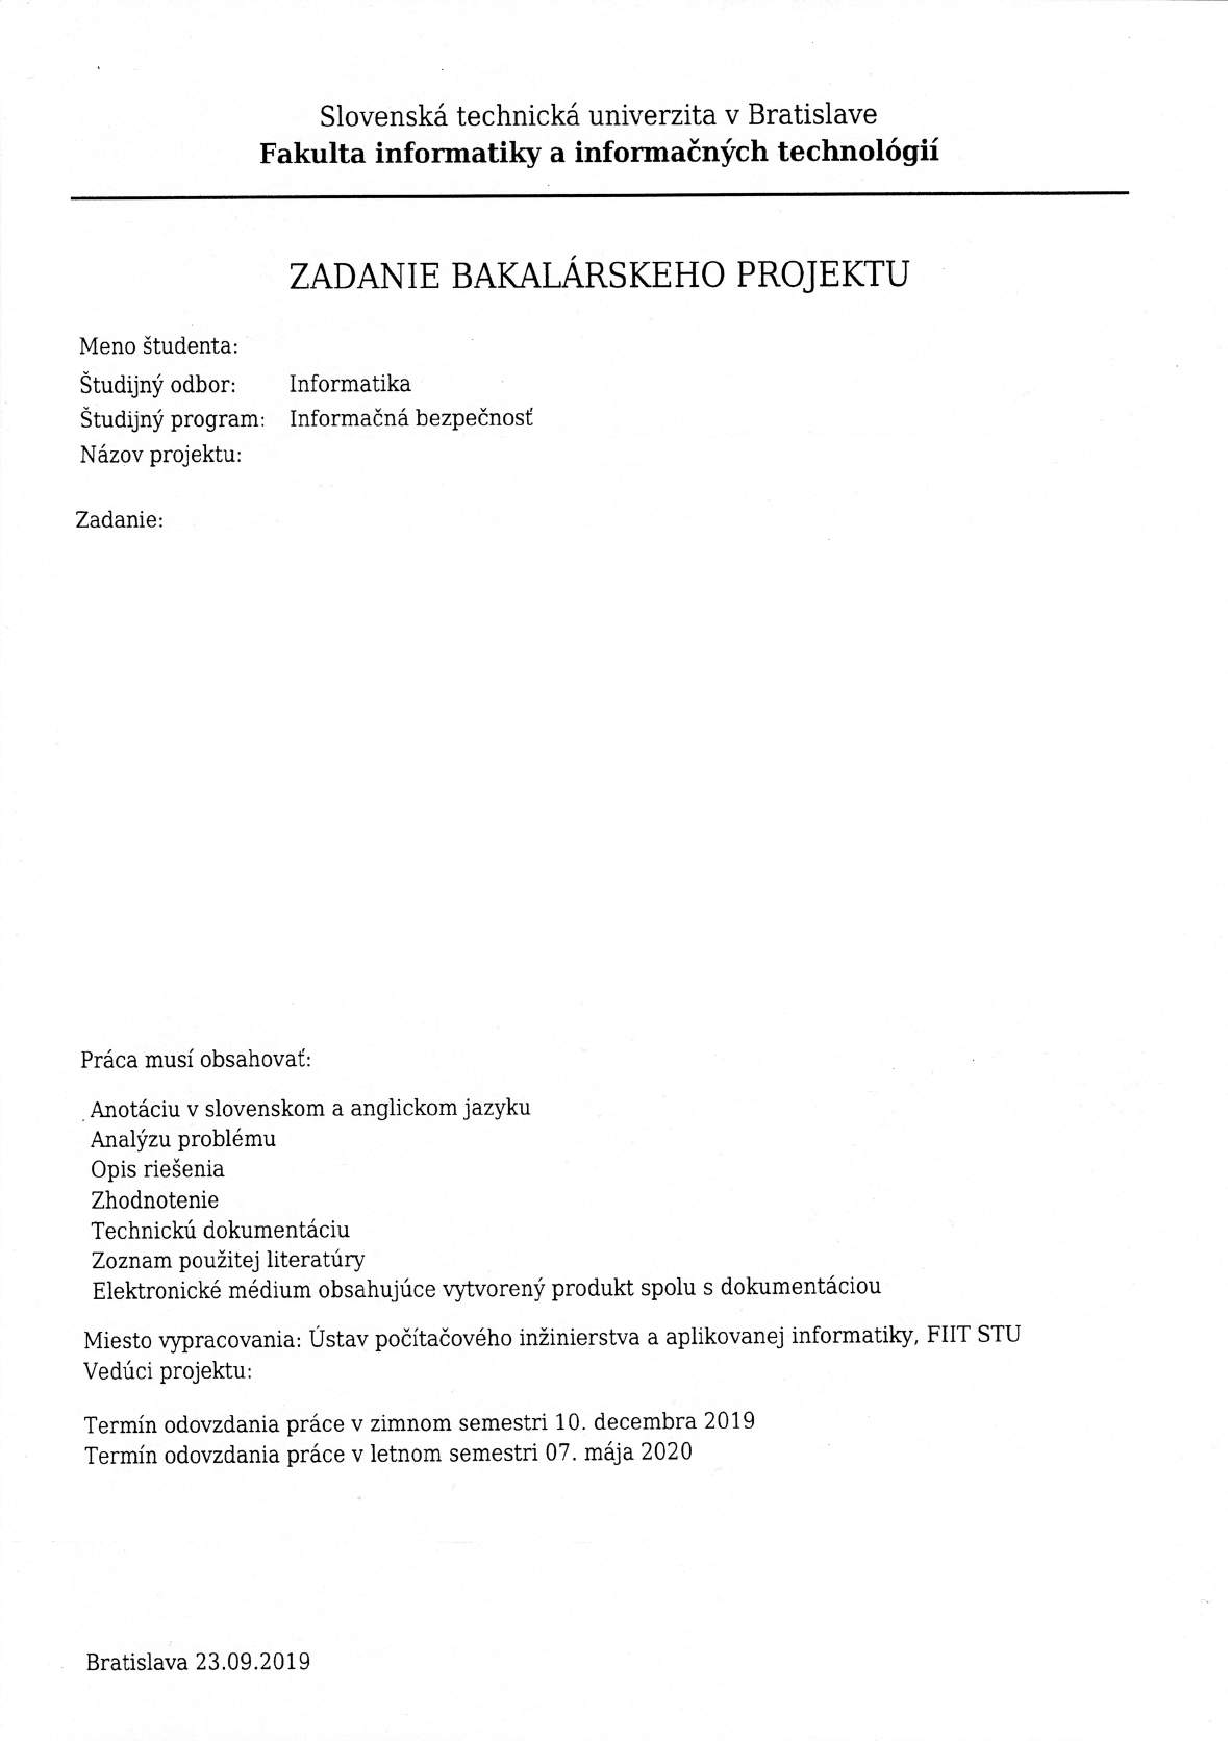
\includepdf[pages=1]{assets/zadanie}
\newpage
\emptypage

% Declaration of honor
\thispagestyle{empty}

\vspace*{\fill}

\ifx\FIITlagEN\undefined
\section*{Čestné prehlásenie}
\else
\section*{Declaration of honor}
\fi

\lorem{1}

\ifx\FIITlagEN\undefined
\FIITsignPlaceSK \FIITsignDate
\else
\FIITsignPlace \FIITsignDate
\fi
\hspace*{\fill} \signaturespace{5cm}{\FIITauthor}

\emptypage

% Acknowledgements
\thispagestyle{empty}

\vspace*{\fill}

\ifx\FIITlagEN\undefined
\section*{Poďakovanie}
\else
\section*{Special thanks}
\fi

\lorem{1}

\newpage
\thispagestyle{empty}
\mbox{}
\newpage

% Table of contents
\ifx\FIITlagEN\undefined
\renewcommand{\contentsname}{Obsah}
\else
\renewcommand{\contentsname}{Table of contents}
\fi
\tableofcontents{}
\emptypage

% List of figures
%\listoffigures
%\emptypage

% List of tables
%\listoftables
%\emptypage

% List of abbreviations
\thispagestyle{plain}

\ifx\FIITlagEN\undefined
\section*{\Huge Zoznam použitých skratiek}
\else
\section*{\Huge List of abbreviations used}
\fi
\vskip 1cm

\begin{tabular}{ >{\bfseries}m{2cm} m{10cm} }
API		& Application Programming Interface \\
AWS		& Amazon Web Services \\
CNAME	& Canonical Name record \\
CSV		& Comma-Separated Values \\
DNS		& Domain Name System \\
HTTP	& Hyper-Text Transfer Protocol \\
ICANN	& Internet Corporation for Assigned Names and Numbers \\
IMAP	& Internet Message Access Protocol \\
IP		& Internet Protocol \\
JSON	& JavaScript Object Notation \\
MD5		& Message-Digest algorithm, version 5 \\
MSSQL	& Microsoft SQL \\
MX		& Mail Exchanger record \\
MySQL	& Maria SQL  \\
NS		& Name Server \\
OS		& Operating System \\
S3		& Amazon Simple Storage Service \\
SHA1	& Secure Hash Algorithm 1 \\
SMTP	& Simple Mail Transfer Protocol \\
SQL		& Structured Query Language \\
SRV		& Service record \\
TLD		& Top-Level Domain \\
URL		& Unified Resource Locator \\
XML		& Extensible Markup Language   
\end{tabular}

\newpage
\thispagestyle{empty}
\mbox{}
\newpage

% Enable page numbering
\pagenumbering{arabic}

% Begin refferences segment
\begin{refsegment}

\chapter{Introduction}
\lipsum[3]
\cite{coplienOredevDCI}

\lipsum[8]
\cite{coplienGOTODCI}
\lipsum[6]
\lipsum[5]

\chapter{Analysis}
\lipsum[3]
\cite{coplienAOSDObjects}

\section{Subsection 1}
\lipsum[8]
\cite{opensourceArch}

\section{Subsection 2}
\lipsum[6]
\lipsum[5]
\cite{generativeProg}

% Bibliography
\printbibliography[heading=references,segment=\therefsegment]

\end{refsegment}
\end{document}
